%%%%%%%%%%%%%%%%%%%%%%%%%%%%%%%%%%%%%%%%%%%%%%%%%%%%%%%%%%%%%%
% --> ENUNCIADO
%%%%%%%%%%%%%%%%%%%%%%%%%%%%%%%%%%%%%%%%%%%%%%%%%%%%%%%%%%%%%%
\section{Enunciado}
El objetivo de este proyecto es familiarizar al estudiante con la programación forma de una estructura de datos básica y/o algoritmo en el lenguaje C++, así como su análisis y presentación. Particularmente en este proyecto se crearan imágenes digitales a partir de archivos binarios.

Se deben tomar archivos binarios de cualquier  índole y calcular el tamaño máximo que puede crearse con sus bytes una imagen X × Y píxeles (no necesariamente cuadrada), tomando en cuenta que cada píxel de dicha imagen esta representado por 3 bytes que representan intensidad de colores rojo, verde y azul, cuyos valores varían entre 0 y 255. Su programa debe tener la capacidad de escribir imágenes en formatos PNG, JPEG, GIF, BMP. Puede utilizar bibliotecas de terceros para implementar esta ultima funcionalidad.
%%%%%%%%%%%%%%%%%%%%%%%%%%%%%%%%%%%%%%%%%%%%%%%%%%%%%%%%%%%%%%
% --> RESEÑA DEL ALGORITMO/ESTRUCTURA
%%%%%%%%%%%%%%%%%%%%%%%%%%%%%%%%%%%%%%%%%%%%%%%%%%%%%%%%%%%%%%
\section{Reseña del algoritmo/estructura}

Una imagen digital en formato RGB se forma por combinación de tres canales. Cada canal se corresponde con un color primario: Red (rojo), Green (verde), y Blue (azul), en donde se asigna un valor de intensidad a cada color que oscila entre 0 y 255, por lo que cada valor de color debe ser guardo en 8 bits o un byte. De la combinación surgen hasta 16,7 millones de colores, que son capaces de describir la mayoría de las imágenes a nivel digital.

En la figura \ref{fig:matrizRGB}, se puede observar con mayor claridad este concepto.

\begin{figure}[H]
\centering
\includegraphics[width=0.6\textwidth]{imgs/proyecto0/matrix.png}
\caption{Imágenes en formato PNG}
\label{fig:matrizRGB}
\end{figure}

Existen en la actualidad una gran cantidad de formatos de archivo que permiten visualizar imágenes digitales que utilizan el mapeo RGB. Esto permite que sea posible implementar algún método que convierta un archivo binario, extrayendo su información en forma de bits puros, mapearlo a RGB, y presentarlo en uno de estos  estándar, de manera que se pueda visualizar con algún dispositivo digital capaz de abrir la imagen. Entre los estándares más comunes se encuentran BMP, PNG, JPG y GIF.

%ESTO SUENA RARO, VOY A TRATAR DE REFRASEARLO   Para generar estas imágenes a partir de un archivo binario de 1 y 0, existen en la actualidad una gran cantidad de formatos de imágenes que nos permite pasar de un archivo binario a una imagen con un formato estándar el cual se puede visualizar con algún dispositivo digital capaz de abrir la imagen con un formato especifico>>> NO LO SÉ, RICK. Entre los estándares más comunes se encuentran BMP, PNG, JPG y GIF. 

A continuación se presenta una breve descripción de las características básicas de los distintos formatos de imagénes que se pretenden usar en este proyecto:

\begin{itemize}
    \item \textbf{PNG}: Las imágenes \textit{Portable Network Graphics}, según \cite{R2} es un formato de imagen sin pérdida que se publicó en 1996. PNG no se diseñó para uso profesional, sino para transferir imágenes en Internet, y solo admite imágenes de nivel de grises e imágenes rgb (también imágenes de color basadas en paletas).
    %---------------------------------------------------------------------
    \item \textbf{JPEG}: Los archivos en formato \textit{Joint Photographic Experts Group}, según \cite{R2} es un formato de imagen que fue aprobado como estándar internacional en 1994. JPEG es usualmente con pérdida, pero también puede ser sin pérdida y se ha convertido en un formato popular para la representación de imágenes en Internet. El estándar define tanto los algoritmos para codificar y decodificar como formato de almacenamiento. JPEG divide la imagen en bloques de 8 × 8 y transforma cada bloquear con una Transformada de Coseno Discreta. Estos valores corresponden a valores más altos 359 frecuencias (variaciones rápidas de color) se establecen en 0 a menos que sean bastante grande, ya que esto no se nota mucho por la percepción humana. Los valores DCT perturbados luego están codificados por una variación de la codificación de Huffman. JPEG también puede usar aritmética codificación, pero esto aumenta los tiempos de codificación y decodificación, con solo alrededor del $\percent[5]$ de mejora en la relación de compresión. El nivel de compresión en imágenes JPEG es seleccionado por el usuario y puede resultar en artefactos conspicuos
    si está configurado demasiado alto. JPEG es especialmente propenso a artefactos en áreas donde la intensidad cambia rápidamente de píxel a píxel. La extensión de un archivo JPEG es .jpg o .jpeg
    %---------------------------------------------------------------------
    \item \textbf{GIF}: El formato \textit{Graphics Interchange Format} fue desarrollado en 1987 por CompuServe Incorporated, principalmente para su uso en Internet. Según \cite{R3}, este formato admite profundidades de color de 1 bit (monocromo) a 8 bits (256 colores) y almacena siempre las imágenes en forma comprimida, utilizando compresión LZW sin pérdida. Otras características compatibles incluyen entrelazado y transparencia.
    %---------------------------------------------------------------------
    \item \textbf{BMP}: El formato \textit{BitMap} fue desarrollado por Microsoft como el formato nativo del sistema operativo Windows. Las versiones del formato han coincidido con las versiones de Windows, la primera versión que aparece en 1985 con Windows 1.0. Según \cite{R3} es un formato  que admite profundidades de color de 1 bit a 32 bits y proporciona compresión RLE opcional sin pérdida.
\end{itemize}

En el cuadro \ref{T:T111}, se muestra un resumen de los distintos formatos: 

\begin{table}[H]
\begin{center}
    \begin{tabular}{ |>{\centering\arraybackslash}m{4cm}|>{\centering\arraybackslash}m{5.5cm}|>{\centering\arraybackslash}m{5.5cm}| }
    	\hline
    	\cellcolor{cl} \textbf{Formato} & \cellcolor{cl} \textbf{Ventajas} & \cellcolor{cl} \textbf{Desventajas}\\ \hline \hline
    	PNG (\textit{Portable Network Graphics}) & Es mejor cuando la imagen tiene grandes áreas uniformemente coloreadas; robusto& Muchos navegadores antiguos actualmente no son compatibles con el formato de archivo PNG. \\
    	\hline
    	JPEG (\textit{Joint Photographic Experts Group}) & Pequeños archivos: la compresión no afecta de manera apreciable la calidad de la imagen & - \\
    	\hline
    	GIF (\textit{Graphics Interchange Format}) & Soporta animaciones & Limitado a 256 colores, sin función real en comparación con otros formatos.\\
    	\hline
    	BMP (\textit{BitMap}) &Son ampliamente usados en los programas de Windows&Son archivos grandes y sin comprimir.\\
    	\hline
    \end{tabular}
\end{center}
\label{T:T111}
\caption{Resumen de características de los formatos de imágenes. \cite{R1}}
\end{table}


%%%%%%%%%%%%%%%%%%%%%%%%%%%%%%%%%%%%%%%%%%%%%%%%%%%%%%%%%%%%%%
% --> FUNCIONAMIENTO DEL ALGORITMO
%%%%%%%%%%%%%%%%%%%%%%%%%%%%%%%%%%%%%%%%%%%%%%%%%%%%%%%%%%%%%%
\section{Funcionamiento del algoritmo/estructura}
El programa se constituye de cuatro clases, una principal encargada de la lectura y apertura del archivo, y tres clases más encargadas de la escritura en determinado formato.
%------------------------------
\subsection{Clase Base \texttt{Pixeles}}
%------------------------------
La clase base \texttt{Pixeles} es a encargada de la apertura y lectura del archivo a trabajar. El método más importante es el encargado de abrir el archivo binario, a esta función le denominamos \texttt{void OpenBinary(const char * path)}, la cual recibe la ruta del archivo a leer. Además de las funciones la clase tiene tres variables protegidas para almacenar el largo y el ancho de la imagen, y una tercera variable que se encarga de almacenar el arreglo en formato RGB que se extrae del binario.

\begin{minted}[linenos,autogobble,bgcolor=bg,breaklines,fontsize=\footnotesize ]{c++}
class Pixeles
{
  public:
    Pixeles();
	void setDimensions(long double size);
    void OpenBinary(const char * path);
    int GetWidth();
    int GetHeight();
    unsigned char * GetArrayRGB();
    ~Pixeles();
  protected:
  private:
    unsigned char * m_pInputImage;
    int m_iWidth;
    int m_iHeight;
};
\end{minted}

\subsubsection{Métodos de \texttt{Pixeles}}
\begin{itemize}
    \item \textbf{Método constructor:} El método constructor para esta clase crea un objeto con los parámetros de largo y ancho iniciados en cero.
    \item \textbf{Método destructor:} Este método destruye el objeto creado y libera la memoria reservada para el arreglo RGB.
    \item \textbf{setDimensions(long double size):} Esta función en la encargada de calcular las dimensiones de la imagen, el formato utilizado fue de 1:1, es decir una imagen cuadrada, por lo tanto solo se necesita calcular la raíz cuadrada del tamaño del arreglo.
    
    \begin{minted}[linenos,autogobble,bgcolor=bg,breaklines,fontsize=\footnotesize ]{c++}
void Pixeles::setDimensions(long double size)
{
	int sqroot;
	sqroot = sqrt(size);
	cout << "la raiz es: " << sqroot << endl;
    this->m_iWidth = sqroot;
    this->m_iHeight = sqroot;
}
\end{minted}

    \item \textbf{Métodos que retornan las variables de la clase:} Como se mencionó anteriormente, la clase utiliza tres variables globales, para obtener estos valores se crearon tres funciones con un simple \texttt{return} de cada tipo.
    
    \begin{minted}[linenos,autogobble,bgcolor=bg,breaklines,fontsize=\footnotesize ]{c++}
int Pixeles::GetWidth(){ return this->m_iWidth;}
int Pixeles::GetHeight(){ return this->m_iHeight;}
unsigned char * Pixeles::GetArrayRGB(){ return this->m_pInputImage;}
\end{minted}
    \item \textbf{void OpenBinary(const char * path):} Este es el método más importante de la clase porque es el encargado de abrir y leer el binario. Este método recibe la ruta del archivo a leer y se encarga de abrirlo y almacenar los datos de interés. Para esto se utiliza un objeto de tipo \texttt{FILE}, con el cual se pueden utilizar las funciones \texttt{fread()}, \texttt{fseek()},\texttt{fputs()} y \texttt{ftell()} para leer el archivo y guardar los datos requeridos en la variable \texttt{m\_pInputImage}, así como para obtener el tamaño del archivo y las dimensiones. Es importante destacar que el arreglo \texttt{m\_pInputImage} se compone de datos tipo \texttt{unsigned char}, es decir bits con valores de 0 a 255. Además, no está de más recordar que toda la memoria reservada se libera al final de la ejecución.
    
    \begin{minted}[linenos,autogobble,bgcolor=bg,breaklines,fontsize=\footnotesize ]{c++}
void Pixeles::OpenBinary(const char * filename)
{
  FILE * pFile;
  unsigned long lSize;
  char * buffer;
  size_t result;

  pFile = fopen ( filename, "rb" );
  if (pFile==NULL) {fputs ("File error",stderr); exit (1);}

  fseek (pFile , 0 , SEEK_END);
  lSize = ftell (pFile);
  rewind (pFile);
  
  long double cantPixeles = lSize/3;
  setDimensions(cantPixeles);

  buffer = new char [lSize];
  if (buffer == NULL) {fputs ("Memory error",stderr); exit (2);}

  result = fread (buffer,1,lSize,pFile);
  if (result != lSize) {fputs ("Reading error",stderr); exit (3);}

  this->m_pInputImage = new unsigned char[this->m_iWidth*this->m_iHeight*3];

  for(long i = 0; i<this->m_iWidth*this->m_iHeight*3; i++)
  {
    this->m_pInputImage[i] = (unsigned char)buffer[i];
    //cout<< +this->m_pInputImage[i] <<endl;
  }
  fclose (pFile);
  delete [] buffer;
}
    \end{minted}
    
\end{itemize}
%Las clases derivadas deben ser capaces 

%------------------------------
\subsection{Clas BMP} 
%------------------------------

Esta clase tiene atributos que definen la altura y el ancho de la imagen a generar, y métodos que se encargan dar formato al arreglo de datos generado por la clase pixeles para convertirlo en una imagen en formato BMP, lacual se guarda en una ruta especificada por el string \texttt{filename}. Según la investigación realizada, para lograr esto se deben definir los atributos necesarios del header de un archivo en formato BMP (metadatos).

En este caso no es necesario usar una biblioteca de terceros, ya que todas las funciones necesarias se encuentran dentro de las librería estándar de C++, esto se puede ya que este formato no hace de ningún método de compresión de los datos para generar la imagen. 

\begin{minted}[linenos,autogobble,bgcolor=bg,breaklines,fontsize=\footnotesize ]{c++}
class BMP
{
  public:
    BMP(int width, int heigh);
    BMP(int width, int height, unsigned char * arrayRGB);
    BMP(const BMP &copyBMP);
    void ReadRGBImageFromBMPFile(string filename);
    unsigned char * GetArrayRGB();
    void SetArrayRGB(unsigned char * arrayRGB);
    bool SaveRGBImageInBMPFile(string filename);
    ~BMP();
  protected:
  private:
    unsigned char * m_pInputImage; /* Array with data RGB of the image */
    char m_sType[2];       /* "BM" */
    int m_iFileSize;       /* Size of file in bytes */
    int m_iReserved;       /* set to 0 */
    int m_iOffBits;        /* Byte offset to actual bitmap data (= 54) */
    int m_iSize;           /* Size of BITMAPINFOHEADER, in bytes (= 40) */
    int m_iWidth;          /* Width of image, in pixels */
    int m_iHeight;         /* Height of images, in pixels */
    short m_sPlanes;       /* Number of planes in target device (set to 1) */
    short m_sBitCount;     /* Bits per pixel (24 in this case) */
    int m_iCompression;    /* Type of compression (0 if no compression) */
    int m_iSizeImage;      /* Image size, in bytes (0 if no compression) */
    int m_iXPelsPerMeter;  /* Resolution in pixels/meter of display device */
    int m_iYPelsPerMeter;  /* Resolution in pixels/meter of display device */
    int m_iClrUsed;        /* Number of colors in the color table (if 0, use
                           maximum allowed by BitCount) */
    int m_iClrImportant;   /* Number of important colors.  If 0, all colors
                           are important */
};
\end{minted}

Esta clase tiene dos constructores con parámetros y un constructor por copia, además de un método llamado \texttt{SaveRGBImageInBMPFile()} que se encarga de generar y almacenar la imagen creada a partir de un arreglo creado por otro método, \texttt{SetArrayRGB()}, el cual tiene un formato tal que sus elementos constituyen los valores de 0 a 255, en binario, en secuencia R-G-B-R-G-B-R...

\begin{minted}[linenos,autogobble,bgcolor=bg,breaklines,fontsize=\footnotesize ]{c++}
void BMP::SetArrayRGB(unsigned char * arrayRGB)
{
  if (sizeof(this->m_pInputImage) != sizeof(arrayRGB)){
    cout<< "Error: Couldn't set array RGB, because it has different dimensions."<<endl;
    return;
  }

  for (int i = 0; i<this->m_iHeight; i++){
      for (int j = 0; j<this->m_iWidth * 3; j += 3){
          int index = (i * this->m_iWidth * 3) + (j);
          this->m_pInputImage[index + 0] = arrayRGB[index + 0];
          this->m_pInputImage[index + 1] = arrayRGB[index + 1];
          this->m_pInputImage[index + 2] = arrayRGB[index + 2];
      }
  }
}
\end{minted}

La creación del archivo de imagen se basa en un objeto del tipo \texttt{FILE}, que se usa como un stream de salida en modo \texttt{"wb"} (\textit{write binary}), y utilizando la función \texttt{fwrite} se guardan en este stream los bytes individualmente, comenzando por los metadatos, seguido de los datos del arreglo anteriormente creado.

\begin{minted}[linenos,autogobble,bgcolor=bg,breaklines,fontsize=\footnotesize ]{c++}
bool BMP::SaveRGBImageInBMPFile(string filename){
  if (this->m_pInputImage==NULL) return 0;
  if (this->m_iWidth==0) return 0;
  if (this->m_iHeight==0) return 0;

  int i, j, jj, ipos;
  int bytesPerLine;
  unsigned char *line;
  unsigned char *ptempImage;

  FILE *file;

  // The length of each line must be a multiple of 4 bytes
  bytesPerLine = (3 * (this->m_iWidth + 1) / 4) * 4;

  strcpy(this->m_sType,"BM");
  this->m_iFileSize = this->m_iOffBits + bytesPerLine*this->m_iHeight;
  this->m_iReserved = 0;
  //(más asignación de variables (metadatos)...)
  this->m_iClrUsed = 0;
  this->m_iClrImportant = 0;

  file = fopen (filename.c_str(), "wb");
  if (file == NULL) return(0);

  fwrite(&this->m_sType, 2, 1, file);
  fwrite(&this->m_iFileSize, 4, 1, file);
  fwrite(&this->m_iReserved, 4, 1, file);
  //(más escritura de metadatos...)
  fwrite(&this->m_iClrUsed, 4, 1, file);
  fwrite(&this->m_iClrImportant, 4, 1, file);

  line = new unsigned char [bytesPerLine];
  if (line == NULL)
  {
      cout<< "Error: Can't allocate memory for BMP file."<<endl;
      return(0);
  }

  //Cambiando posición del sistema de coordenadas de la esquina inferior izquierda a la esquina superior izquierda.
  ptempImage = new unsigned char [this->m_iWidth*this->m_iHeight*3];
  for (i=0;i<this->m_iWidth*this->m_iHeight*3;i++) ptempImage[i]=0;
  jj=0;
  for (j=this->m_iHeight-1;j>=0;j--){
      for (i=0;i<this->m_iWidth;i++){
          ptempImage[jj*3*this->m_iWidth+3*i]= this->m_pInputImage[j*3*this->m_iWidth+3*i];
          ptempImage[jj*3*this->m_iWidth+3*i+1]= this->m_pInputImage[j*3*this->m_iWidth+3*i+1];
          ptempImage[jj*3*this->m_iWidth+3*i+2]= this->m_pInputImage[j*3*this->m_iWidth+3*i+2];
      }
      jj++;
  }

  for (i = this->m_iHeight - 1; i >= 0; i--){
      for (j = 0; j < this->m_iWidth; j++){
          ipos = 3*(this->m_iWidth * i + j);
          line[3*j] = ptempImage[ipos+2];
          line[3*j+1] = ptempImage[ipos+1];
          line[3*j+2] = ptempImage[ipos];
      }
      fwrite(line, bytesPerLine, 1, file);
  }
  delete [] line;
  fclose(file);
  delete [] ptempImage;
  return(1);
}

\end{minted}

%------------------------------
\subsection{Clase PNG}
%------------------------------

Para la clase PNG se utilizó la biblioteca \texttt{libpng}, la cual se incluyó mediante el encabezado \texttt{\#include <png.h>}. Esta clase se constituye de varios métodos y variables, en donde destaca el método \texttt{bool SaveRGBImageInPNGFile(string filename, const char *title)} encargado de crear la imagen en formato PNG a partir de una entrada RGB.

\begin{minted}[linenos,autogobble,bgcolor=bg,breaklines,fontsize=\footnotesize ]{c++}
class PNG
{
  public:
    PNG(int width, int height);
    PNG(int width, int height, unsigned char * arrayRGB);
    PNG(const PNG &copyPNG);
    unsigned char * GetArrayRGB();
    void SetArrayRGB(unsigned char * arrayRGB);
    bool SaveRGBImageInPNGFile(string filename, const char *title);
    ~PNG();
  protected:
  private:
    unsigned char * m_pInputImage; /* Array with data RGB of the image */
    int m_iWidth;          /* Width of image, in pixels */
    int m_iHeight;         /* Height of images, in pixels */
};
\end{minted}

\subsubsection{Métodos de \texttt{PNG}}
\begin{itemize}
    \item \textbf{Métodos constructores:} La clase posee dos constructores distintos, uno recibe únicamente los valores del largo y el ancho de la imagen, y el otro constructor recibe además el arreglo RGB que se va a utilizar. Ambos métodos reservan la memoria necesaria para ese arreglo que se va a trabajar.
    
    \begin{minted}[linenos,autogobble,bgcolor=bg,breaklines,fontsize=\footnotesize ]{c++}
PNG::PNG(int width, int height)
{
  this->m_iWidth = width;
  this->m_iHeight = height;
  this->m_pInputImage =  new unsigned char[width*height*3];
  cout << "/* constructor png */" << endl;
}
PNG::PNG(int width, int height, unsigned char * arrayRGB)
{
  this->m_iWidth = width;
  this->m_iHeight = height;
  this->m_pInputImage = new unsigned char[width*height*3];
  SetArrayRGB(arrayRGB);
  cout << "/* constructor png */" << endl;
}
    \end{minted}

    \item \textbf{Método para obtener el arreglo RGB:} Se creó un método que simplemente regresa el arreglo RGB.
    
    \item \textbf{void SetArrayRGB(unsigned char * arrayRGB):} Este método se encarga de tomar los valores del arreglo RGB ingresado y copiarlos en el arreglo local que se utiliza para trabajar. Además verifica que la memoria reservada (el tamaño) concuerde.
    
    \begin{minted}[linenos,autogobble,bgcolor=bg,breaklines,fontsize=\footnotesize ]{c++}
void PNG::SetArrayRGB(unsigned char * arrayRGB)
{
  if (sizeof(this->m_pInputImage) != sizeof(arrayRGB))
  {
    cout<< "Error: Couldn't set array RGB, because it has differents dimensions."<<endl;
    return;
  }
  for (int i = 0; i<this->m_iHeight; i++)
  {
      int jj = 0;
      for (int j = this->m_iWidth * 3; j>0; j -= 3)
      {
          int index = (i * this->m_iWidth * 3) + (j);
          int pos = (i * this->m_iWidth * 3) + (jj);
          //cout << (long *)arrayRGB[index + 0]<< '\n';
          this->m_pInputImage[pos + 0] = arrayRGB[this->m_iHeight * this->m_iWidth * 3  - index + 0];
          this->m_pInputImage[pos + 1] = arrayRGB[this->m_iHeight * this->m_iWidth * 3  - index + 1];
          this->m_pInputImage[pos + 2] = arrayRGB[this->m_iHeight * this->m_iWidth * 3  -index + 2];
          jj+=3;
      }
  }
}
    \end{minted}
    
    \item \textbf{bool SaveRGBImageInPNGFile(string filename, const char *title):} Este es el método más importante de la clase debido a que es el que efectivamente va a escribir la imagen deseada. Para este método se utiliza \texttt{FILE} y sus funciones para abrir el archivo y extraer la información. La parte principal del funcionamiento del programa se da mediante el uso de las funciones propias de la biblioteca \texttt{libpng}, como por ejemplo \texttt{png\_init\_io(png\_ptr, fp)} o \texttt{png\_write\_info(png\_ptr, info\_ptr)}. Para la utilización de estos comandos se siguió completamente la documentación de la biblioteca. 
    
     \begin{minted}[linenos,autogobble,bgcolor=bg,breaklines,fontsize=\footnotesize ]{c++}
     
bool PNG::SaveRGBImageInPNGFile(string filename, const char *title)
{
  if (this->m_pInputImage==NULL) return 0;
  if (this->m_iWidth==0) return 0;
  if (this->m_iHeight==0) return 0;

	bool code = 0;
	FILE *fp = NULL;
	png_structp png_ptr = NULL;
	png_infop info_ptr = NULL;
	png_bytep row = NULL;

	// Open file for writing (binary mode)
	fp = fopen(filename.c_str(), "wb");
	if (fp == NULL)
  {
		cout<< "Error: Couldn't open file"<<filename<< "for writing."<<endl;
		code = 1;
		goto finalise;
	}

	// Initialize write structure
	png_ptr = png_create_write_struct(PNG_LIBPNG_VER_STRING, NULL, NULL, NULL);
	if (png_ptr == NULL)
  {
		cout<< "Error: Couldn't allocate write struct."<<endl;
		code = 1;
		goto finalise;
	}

	// Initialize info structure
	info_ptr = png_create_info_struct(png_ptr);
	if (info_ptr == NULL)
  {
    cout<< "Error: Couldn't allocate info struct."<<endl;
		code = 1;
		goto finalise;
	}
	// Setup Exception handling
	if (setjmp(png_jmpbuf(png_ptr)))
  {
		cout <<"Error: Problem during png creation."<<endl;
		code = 1;
		goto finalise;
	}
	png_init_io(png_ptr, fp);
	// Write header (8 bit colour depth)
	png_set_IHDR(png_ptr, info_ptr, this->m_iWidth, this->m_iHeight, 8,
      PNG_COLOR_TYPE_RGB, PNG_INTERLACE_NONE,
			PNG_COMPRESSION_TYPE_BASE, PNG_FILTER_TYPE_BASE);
	// Set title
	if (title != NULL)
  {
		png_text title_text;
		title_text.compression = PNG_TEXT_COMPRESSION_NONE;
		title_text.key = (char *)"Title";
		title_text.text = (char *)title;
		png_set_text(png_ptr, info_ptr, &title_text, 1);
	}

	png_write_info(png_ptr, info_ptr);

	// Allocate memory for one row (3 bytes per pixel - RGB)
	row = (png_bytep) malloc(3 * this->m_iWidth * sizeof(png_byte));

	// Write image data
	//int x, y;
	for (int y=0 ; y<this->m_iHeight ; y++)
  {
		for (int x=0 ; x<this->m_iWidth*3; x+=3)
    {
      int index = (y * this->m_iWidth * 3) + (x);
      row[x+0] = this->m_pInputImage[index + 0];
      row[x+1] = this->m_pInputImage[index + 1];
      row[x+2] = this->m_pInputImage[index + 2];
		}
		png_write_row(png_ptr, row);
	}
	// End write
	png_write_end(png_ptr, NULL);

	finalise:
	if (fp != NULL) fclose(fp);
	if (info_ptr != NULL) png_free_data(png_ptr, info_ptr, PNG_FREE_ALL, -1);
	if (png_ptr != NULL) png_destroy_write_struct(&png_ptr, (png_infopp)NULL);
	if (row != NULL) free(row);
	return code;
}
    \end{minted}
    
\end{itemize}

%------------------------------
\subsection{Clase JPG}
%------------------------------
Esta clase contiene métodos que utilizan la biblioteca \texttt{jpeglib} de trabajar el formato JPEG con su algoritmo de compresión. Toda esta biblioteca está escrita completamente en C. 

Los atributos de la clase JPG son las dimensiones y el arreglo de datos de entrada, y los métodos incluyen uno para generar el arreglo formateado a R-G-B (\texttt{SetArrayRGB()}), y otro (\texttt{SaveRGBImageInJPGFile()}) que hace uso de la funcionalidad de \texttt{jpeglib} para guardar la imagen generada.

\begin{minted}[linenos,autogobble,bgcolor=bg,breaklines,fontsize=\footnotesize ]{c++}
class JPG
{
  public:
    JPG(int width, int height);
    JPG(int width, int height, unsigned char * arrayRGB);
    JPG(const JPG &copyJPG);
    unsigned char * GetArrayRGB();
    void SetArrayRGB(unsigned char * arrayRGB);
    bool SaveRGBImageInJPGFile(string filename, bool color, int quality);
    ~JPG();
  protected:
  private:
    unsigned char * m_pInputImage; /* Array with data RGB of the image */
    int m_iWidth;          /* Width of image, in pixels */
    int m_iHeight;         /* Height of images, in pixels */
};
\end{minted}

Él método \texttt{SetArrayRGB()} funciona exactamente de la misma manera que en las clases anteriores. 

En el caso del método (\texttt{SaveRGBImageInJPGFile()}), se encontró que la documentación de \texttt{jpeglib} es muy completa y facilitó el uso de las funciones para producir la imagen de salida.

\begin{minted}[linenos,autogobble,bgcolor=bg,breaklines,fontsize=\footnotesize ]{c++}
bool JPG::SaveRGBImageInJPGFile(string filename, bool color, int quality){
    unsigned char * tmp;
	if (!color){
	    tmp = (unsigned char*)new unsigned char[this->m_iWidth*this->m_iHeight];
	    if (tmp==NULL){
	        cout<< "Error: Can't allocate memory for JPG file."<<endl;
	        return FALSE;
	    }
	    int row,col;
	    for (row=0; row<this->m_iHeight;row++){
	        for (col=0;col<this->m_iWidth;col++){
	            unsigned char pRed, pGrn, pBlu;
	            pRed = this->m_pInputImage[row * 3 * this->m_iWidth + col * 3 + 0];
	            pGrn = this->m_pInputImage[row * 3 * this->m_iWidth + col * 3 + 1];
	            pBlu = this->m_pInputImage[row * 3 * this->m_iWidth + col * 3 + 2];
	            // luminance
	            int lum = (int)(.299 * (double)(pRed) + .587 * (double)(pGrn) + .114 * (double)(pBlu));
	            unsigned char pGray = (unsigned char)lum;
	            tmp[row * this->m_iWidth + col] = pGray;
	       }
	   }
    }

	struct jpeg_compress_struct cinfo;
	FILE * outfile = NULL;			/* target file */

	/* Step 1: allocate and initialize JPEG compression object */
	cinfo.err = jpeg_std_error(&jerr.pub);
	jerr.pub.error_exit = my_error_exit;

	/* Establish the setjmp return context for my_error_exit to use. */
	if (setjmp(jerr.setjmp_buffer)){ //error code
	   jpeg_destroy_compress(&cinfo);
	   if (outfile!=NULL)
	        fclose(outfile);
	   if (!color){
	        delete [] tmp;
	   }
	return FALSE;
	}

	/* Now we can initialize the JPEG compression object. */
	jpeg_create_compress(&cinfo);

	/* Step 2: specify data destination (eg, a file) */
	if ((outfile = fopen(filename.c_str(), "wb")) == NULL){
	    cout<< "Error: Couldn't open file"<<filename<< "for writing."<<endl;
	    return FALSE;
	}
	jpeg_stdio_dest(&cinfo, outfile);
	/* Step 3: set parameters for compression */

	cinfo.image_width = this->m_iWidth;
	cinfo.image_height = this->m_iHeight;
	if (color){
	    cinfo.input_components = 3;		/* # of color components per pixel */
	    cinfo.in_color_space = JCS_RGB; 	/* colorspace of input image */
	} else {
	    cinfo.input_components = 1;		/* # of color components per pixel */
	    cinfo.in_color_space = JCS_GRAYSCALE; 	/* colorspace of input image */
	}
    jpeg_set_defaults(&cinfo);
    
    jpeg_set_quality(&cinfo, quality, TRUE /* limit to baseline-JPEG values */);
    
    /* Step 4: Start compressor */
    
    /* TRUE ensures that we will write a complete interchange-JPEG file */
    jpeg_start_compress(&cinfo, TRUE);
    
    /* Step 5: while (scan lines remain to be written): jpeg_write_scanlines(...); */
    
    /* Here we use the library's state variable cinfo.next_scanline as the loop counter*/
    while (cinfo.next_scanline < cinfo.image_height){
        unsigned char *outRow;
        if (color){
      		outRow = this->m_pInputImage + (cinfo.next_scanline * this->m_iWidth * 3);
      	} else {
      		outRow = tmp + (cinfo.next_scanline * this->m_iWidth );
      	}
        (void) jpeg_write_scanlines(&cinfo, &outRow, 1);
    }
    
    /* Step 6: Finish compression and close the output file*/
    jpeg_finish_compress(&cinfo);
    fclose(outfile);
    
    /* Step 7: release JPEG compression object */
      jpeg_destroy_compress(&cinfo);
    
      if (!color) delete [] tmp;
  return TRUE;
}

\end{minted}

% PNG -> libjpeg-dev -> sudo apt-get install libjpeg-dev 

%------------------------------
\subsection{Clase GIF}
%------------------------------
Para implementar la escritura en formato GIF se trató de utilizar la biblioteca \texttt{giflib}, pero debido a la mala documentación de la misma, y la escasez de información respecto a ella no se pudo implementar de manera satisfactoria. También se intentó utilizar el paquete \texttt{Magick++} de \texttt{ImageMagick}, pero de igual manera no se logró crear una imagen en formato GIF.

%%%%%%%%%%%%%%%%%%%%%%%%%%%%%%%%%%%%%%%%%%%%%%%%%%%%%%%%%%%%%%
% --> EXPERIMENTOS QUE SE REALIZARAN
%%%%%%%%%%%%%%%%%%%%%%%%%%%%%%%%%%%%%%%%%%%%%%%%%%%%%%%%%%%%%%
\section{Experimentos realizados}

Para ejemplificar la funcionalidad de las clases creadas se realizó un programa principal, que toma como parámetro la ruta del archivo binario que se utiliza como entrada (\textit{filepath}), y a partir del cual se generan las imágenes correspondientes en los 3 formatos implementados. Se crea un objeto de la clase Pixeles, y se ejecuta su método \texttt{OpenBinary(filepath)}, para obtener las dimensiones de la imagen que se puede generar y el arreglo de datos.

Luego se instancian las clases BMP, JPG y PNG para efectivamente crear las imágenes en cada formato, las cuales luego se almacenan en un directorio dado.

Aquí también se incluyó código para medir los tiempos de ejecución en milisegundos de los algoritmos de generación de cada imagen. Para esto, se utiliza la biblioteca \texttt{chrono}, que provee de distintos tipos de relojes (clocks). En este caso, se utilizó el reloj de tipo \texttt{high\_resolution\_clock}, con el cual se hace un \textit{time point} antes y después del segmento de código que se quiere cronometrar. Luego el template \texttt{duration} representa el intervalo de tiempo transcurrido y, con el método \texttt{count()}, se transforma este valor a segundos.


\begin{minted}[linenos,autogobble,bgcolor=bg,breaklines,fontsize=\footnotesize ]{c++}
#include <iostream>
#include <chrono>
#include "../include/bmp.hpp"
#include "../include/png.hpp"
#include "../include/jpg.hpp"
#include "../include/gif.hpp"
#include "../include/pixeles.hpp"

using  namespace std;

int main(int argc, char const *argv[]){
  if (argc == 0){
    cout << "/* Ingrese una ruta del archivo binario */" << '\n';
    return 0;
  }
  const char * filepath = argv[1];
  Pixeles PIX;
  PIX.OpenBinary(filepath);

  cout<<"***************************************************************"<<endl;
  BMP TestBMP(PIX.GetWidth(),PIX.GetHeight(),PIX.GetArrayRGB());

  auto t0 = chrono::high_resolution_clock::now();
  TestBMP.SaveRGBImageInBMPFile("./output/outBMP.bmp");
  auto t1 = chrono::high_resolution_clock::now();
  chrono::duration<double> TimeWriteBMP = t1 - t0;
  cout << "Tiempo ejecución de BMP: " << (TimeWriteBMP.count()*1000) << " ms" << endl;

  cout<<"***************************************************************"<<endl;
  PNG TestPNG(PIX.GetWidth(),PIX.GetHeight(),PIX.GetArrayRGB());

  auto t2 = chrono::high_resolution_clock::now();
  TestPNG.SaveRGBImageInPNGFile("./output/outPNG.png","Test");
  auto t3 = chrono::high_resolution_clock::now();
  chrono::duration<double> TimeWritePNG = t3 - t2;
  cout << "Tiempo ejecución de PNG: " << (TimeWritePNG.count()*1000) << " ms" << endl;

  cout<<"***************************************************************"<<endl;
  JPG TestJPG(PIX.GetWidth(),PIX.GetHeight(),PIX.GetArrayRGB());

  auto t4 = chrono::high_resolution_clock::now();
  TestJPG.SaveRGBImageInJPGFile("./output/outJPG.jpg",1,75);
  auto t5 = chrono::high_resolution_clock::now();
  chrono::duration<double> TimeWriteJPG = t5 - t4;
  cout << "Tiempo ejecución de JPG: " << (TimeWriteJPG.count()*1000) << " ms" << endl;

  cout<<"***************************************************************"<<endl;

  return 0;
}
\end{minted}

Finalmente, se probó la funcionalidad del programa al ejecutar un comando \texttt{make run file = ruta\_de\_archivo\_de\_entrada}, con lo cual fue posible almacenar las imágenes generadas y abrirlas automáticamente. Se realizó este procedimiento pasando como entrada diferentes archivos con extensiones \texttt{.pdf}, \texttt{.o}, \texttt{.mp3} y \texttt{.bmp}.

%%%%%%%%%%%%%%%%%%%%%%%%%%%%%%%%%%%%%%%%%%%%%%%%%%%%%%%%%%%%%%
% --> RESULTADOS OBTENIDOS
%%%%%%%%%%%%%%%%%%%%%%%%%%%%%%%%%%%%%%%%%%%%%%%%%%%%%%%%%%%%%%
\section{Resultados obtenidos}
En las siguientes figuras se observan las imágenes obtenidas al ejecutar el programa utilizando como entrada archivos binarios de diferentes extensiones.

\begin{figure}[H]
\centering
\begin{tabular}{c c c}
\subfloat[Imagen en formato JPG]
{\includegraphics[width=0.3\textwidth]{imgs/proyecto0/boutJPG.jpg}}
&
\subfloat[Imagen en formato PNG]
{\includegraphics[width=0.3\textwidth]{imgs/proyecto0/boutPNG.png}}
&
\subfloat[Imagen en formato BMP]
{\includegraphics[width=0.3\textwidth]{imgs/proyecto0/boutPNG.png}}
\\
\end{tabular}
\caption{Imágenes obtenidas de un binario .o.}
\label{F:oo}
\end{figure}

%salida del pdf


\begin{figure}[H]
\centering
\begin{tabular}{c c c}
\subfloat[Imagen en formato JPG]
{\includegraphics[width=0.3\textwidth]{imgs/proyecto0/outPNG-pdf}}
&
\subfloat[Imagen en formato PNG]
{\includegraphics[width=0.3\textwidth]{imgs/proyecto0/outJPG-pdf}}
&
\subfloat[Imagen en formato BMP]
{\includegraphics[width=0.3\textwidth]{imgs/proyecto0/outPNG-pdf}}
\\
\end{tabular}
\caption{Imágenes obtenidas de un binario .pdf}
\label{F:pdf}
\end{figure}

\begin{figure}[H]
\centering
\begin{tabular}{c c c}
\subfloat[Imagen en formato JPG]
{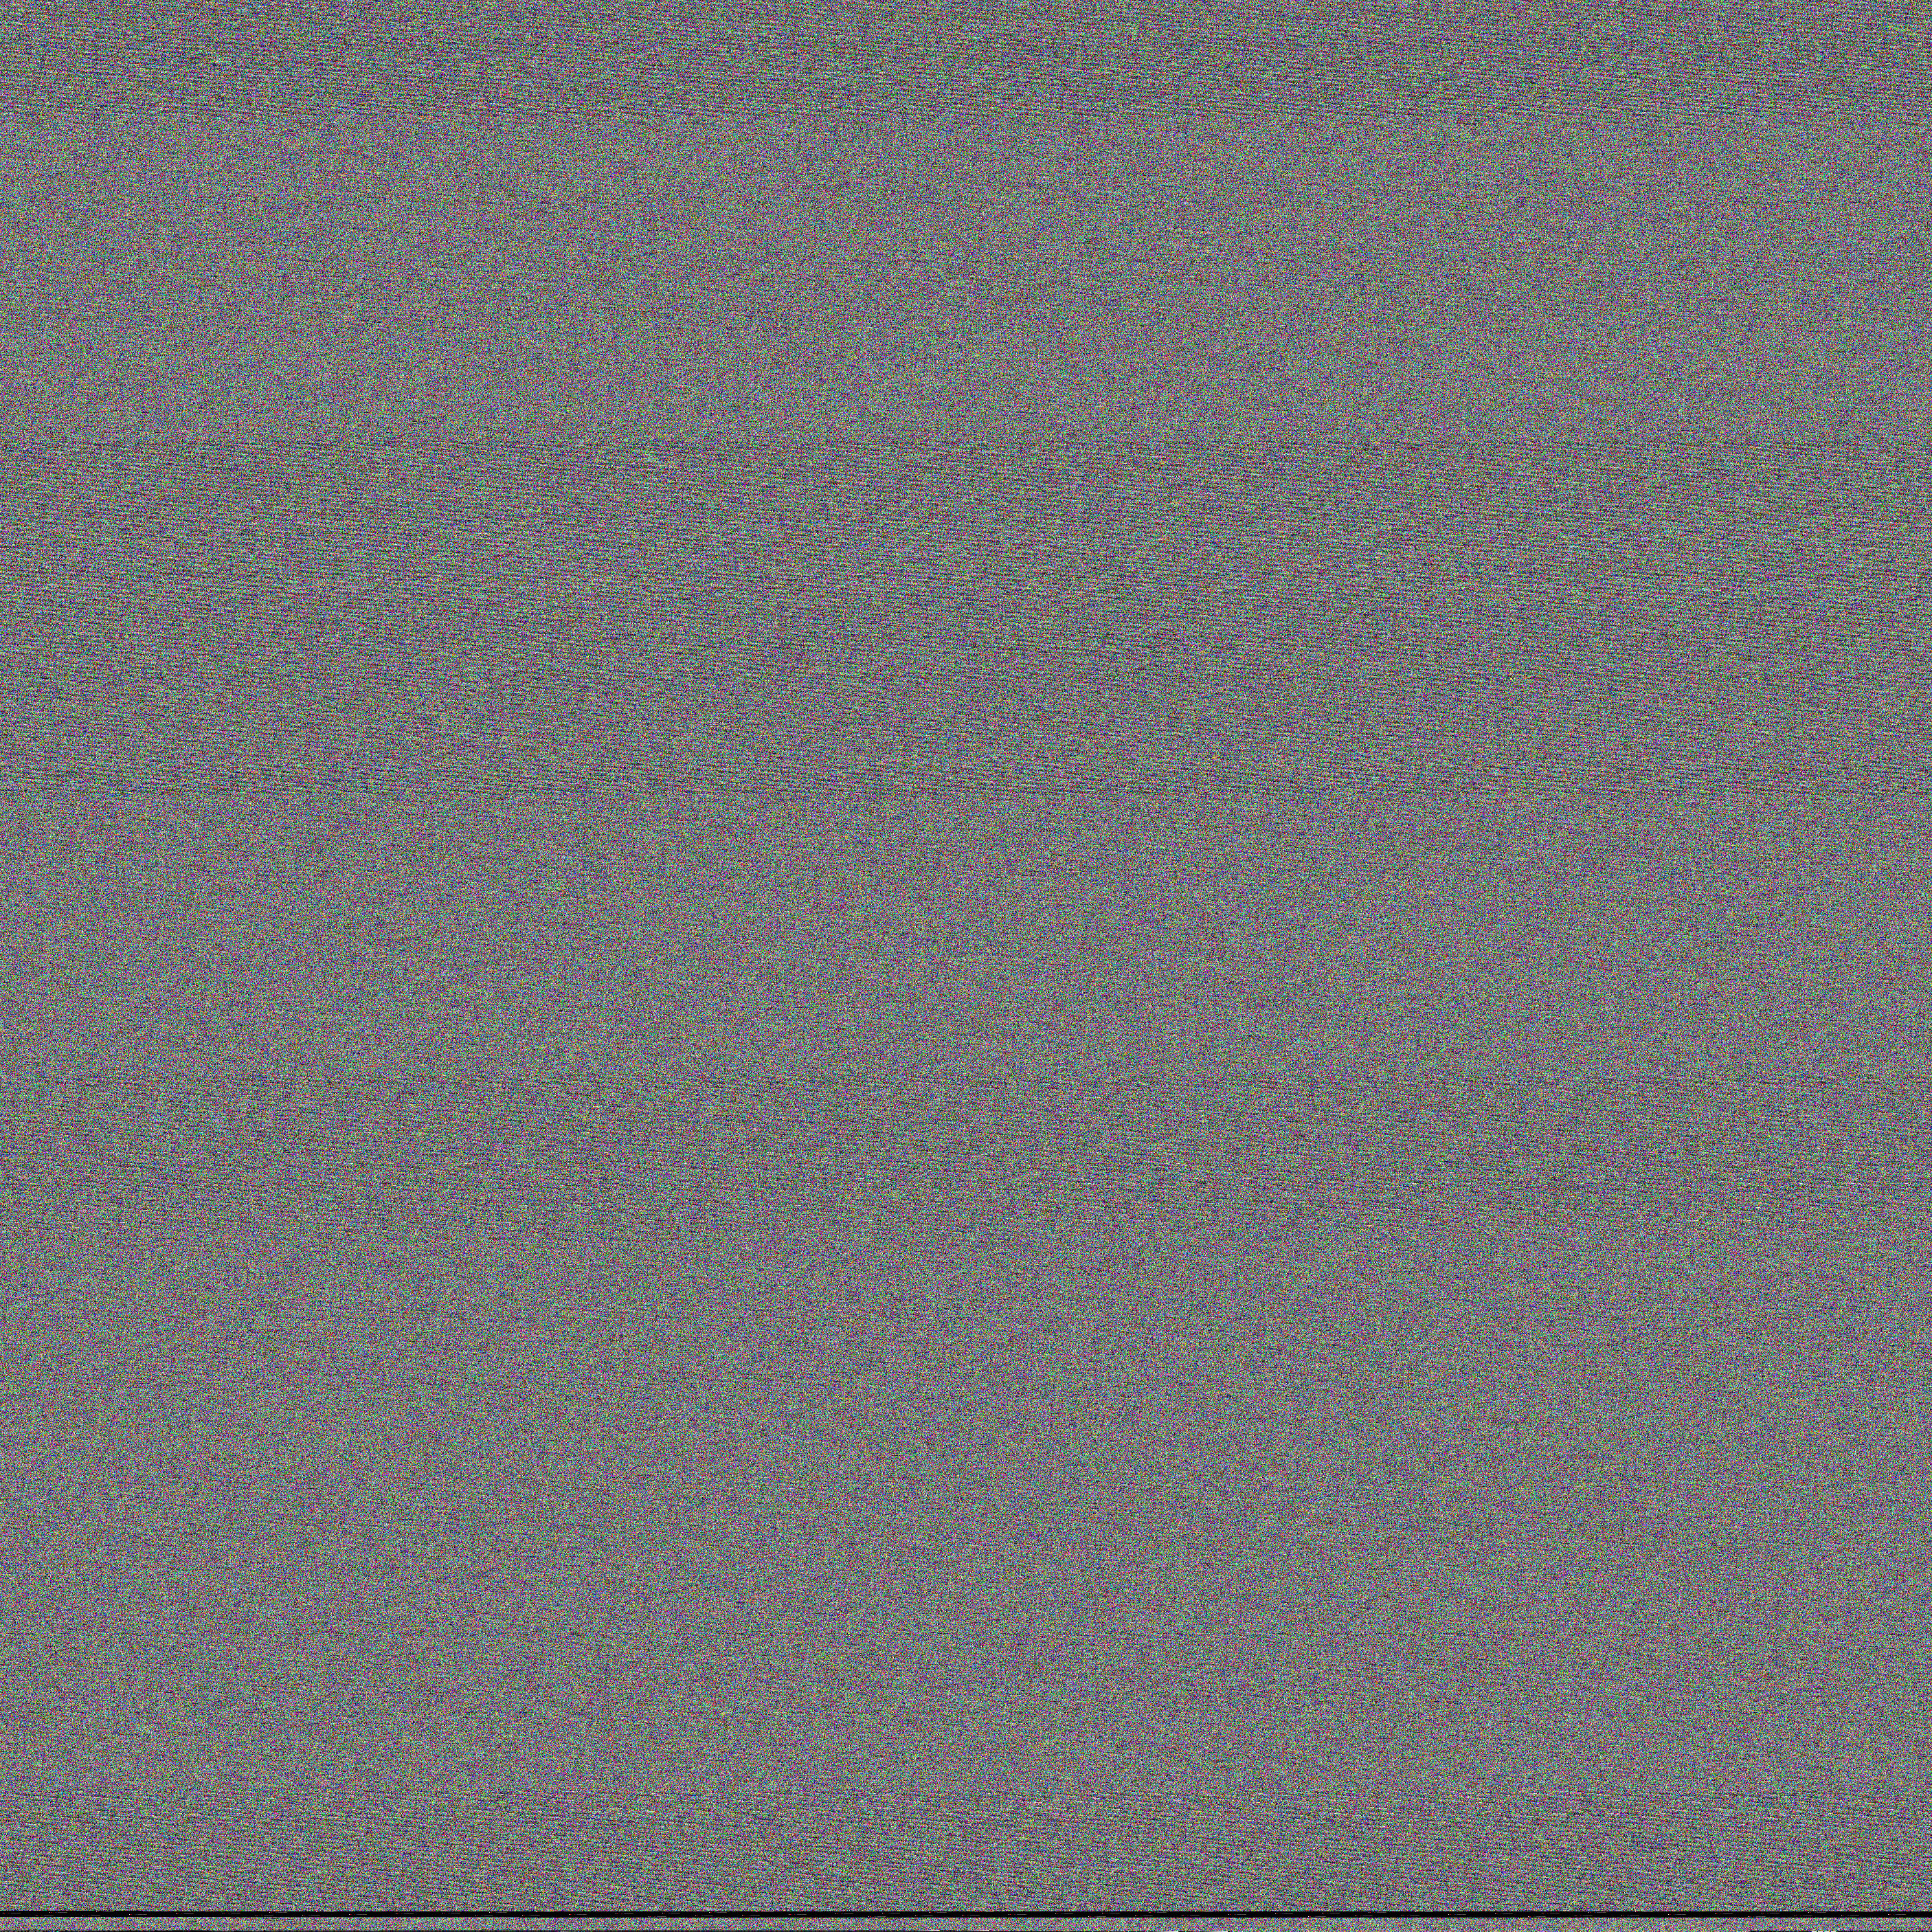
\includegraphics[width=0.3\textwidth]{imgs/proyecto0/outPNG-mp3}}
&
\subfloat[Imagen en formato PNG]
{\includegraphics[width=0.3\textwidth]{imgs/proyecto0/outJPG-mp3}}
&
\subfloat[Imagen en formato BMP]
{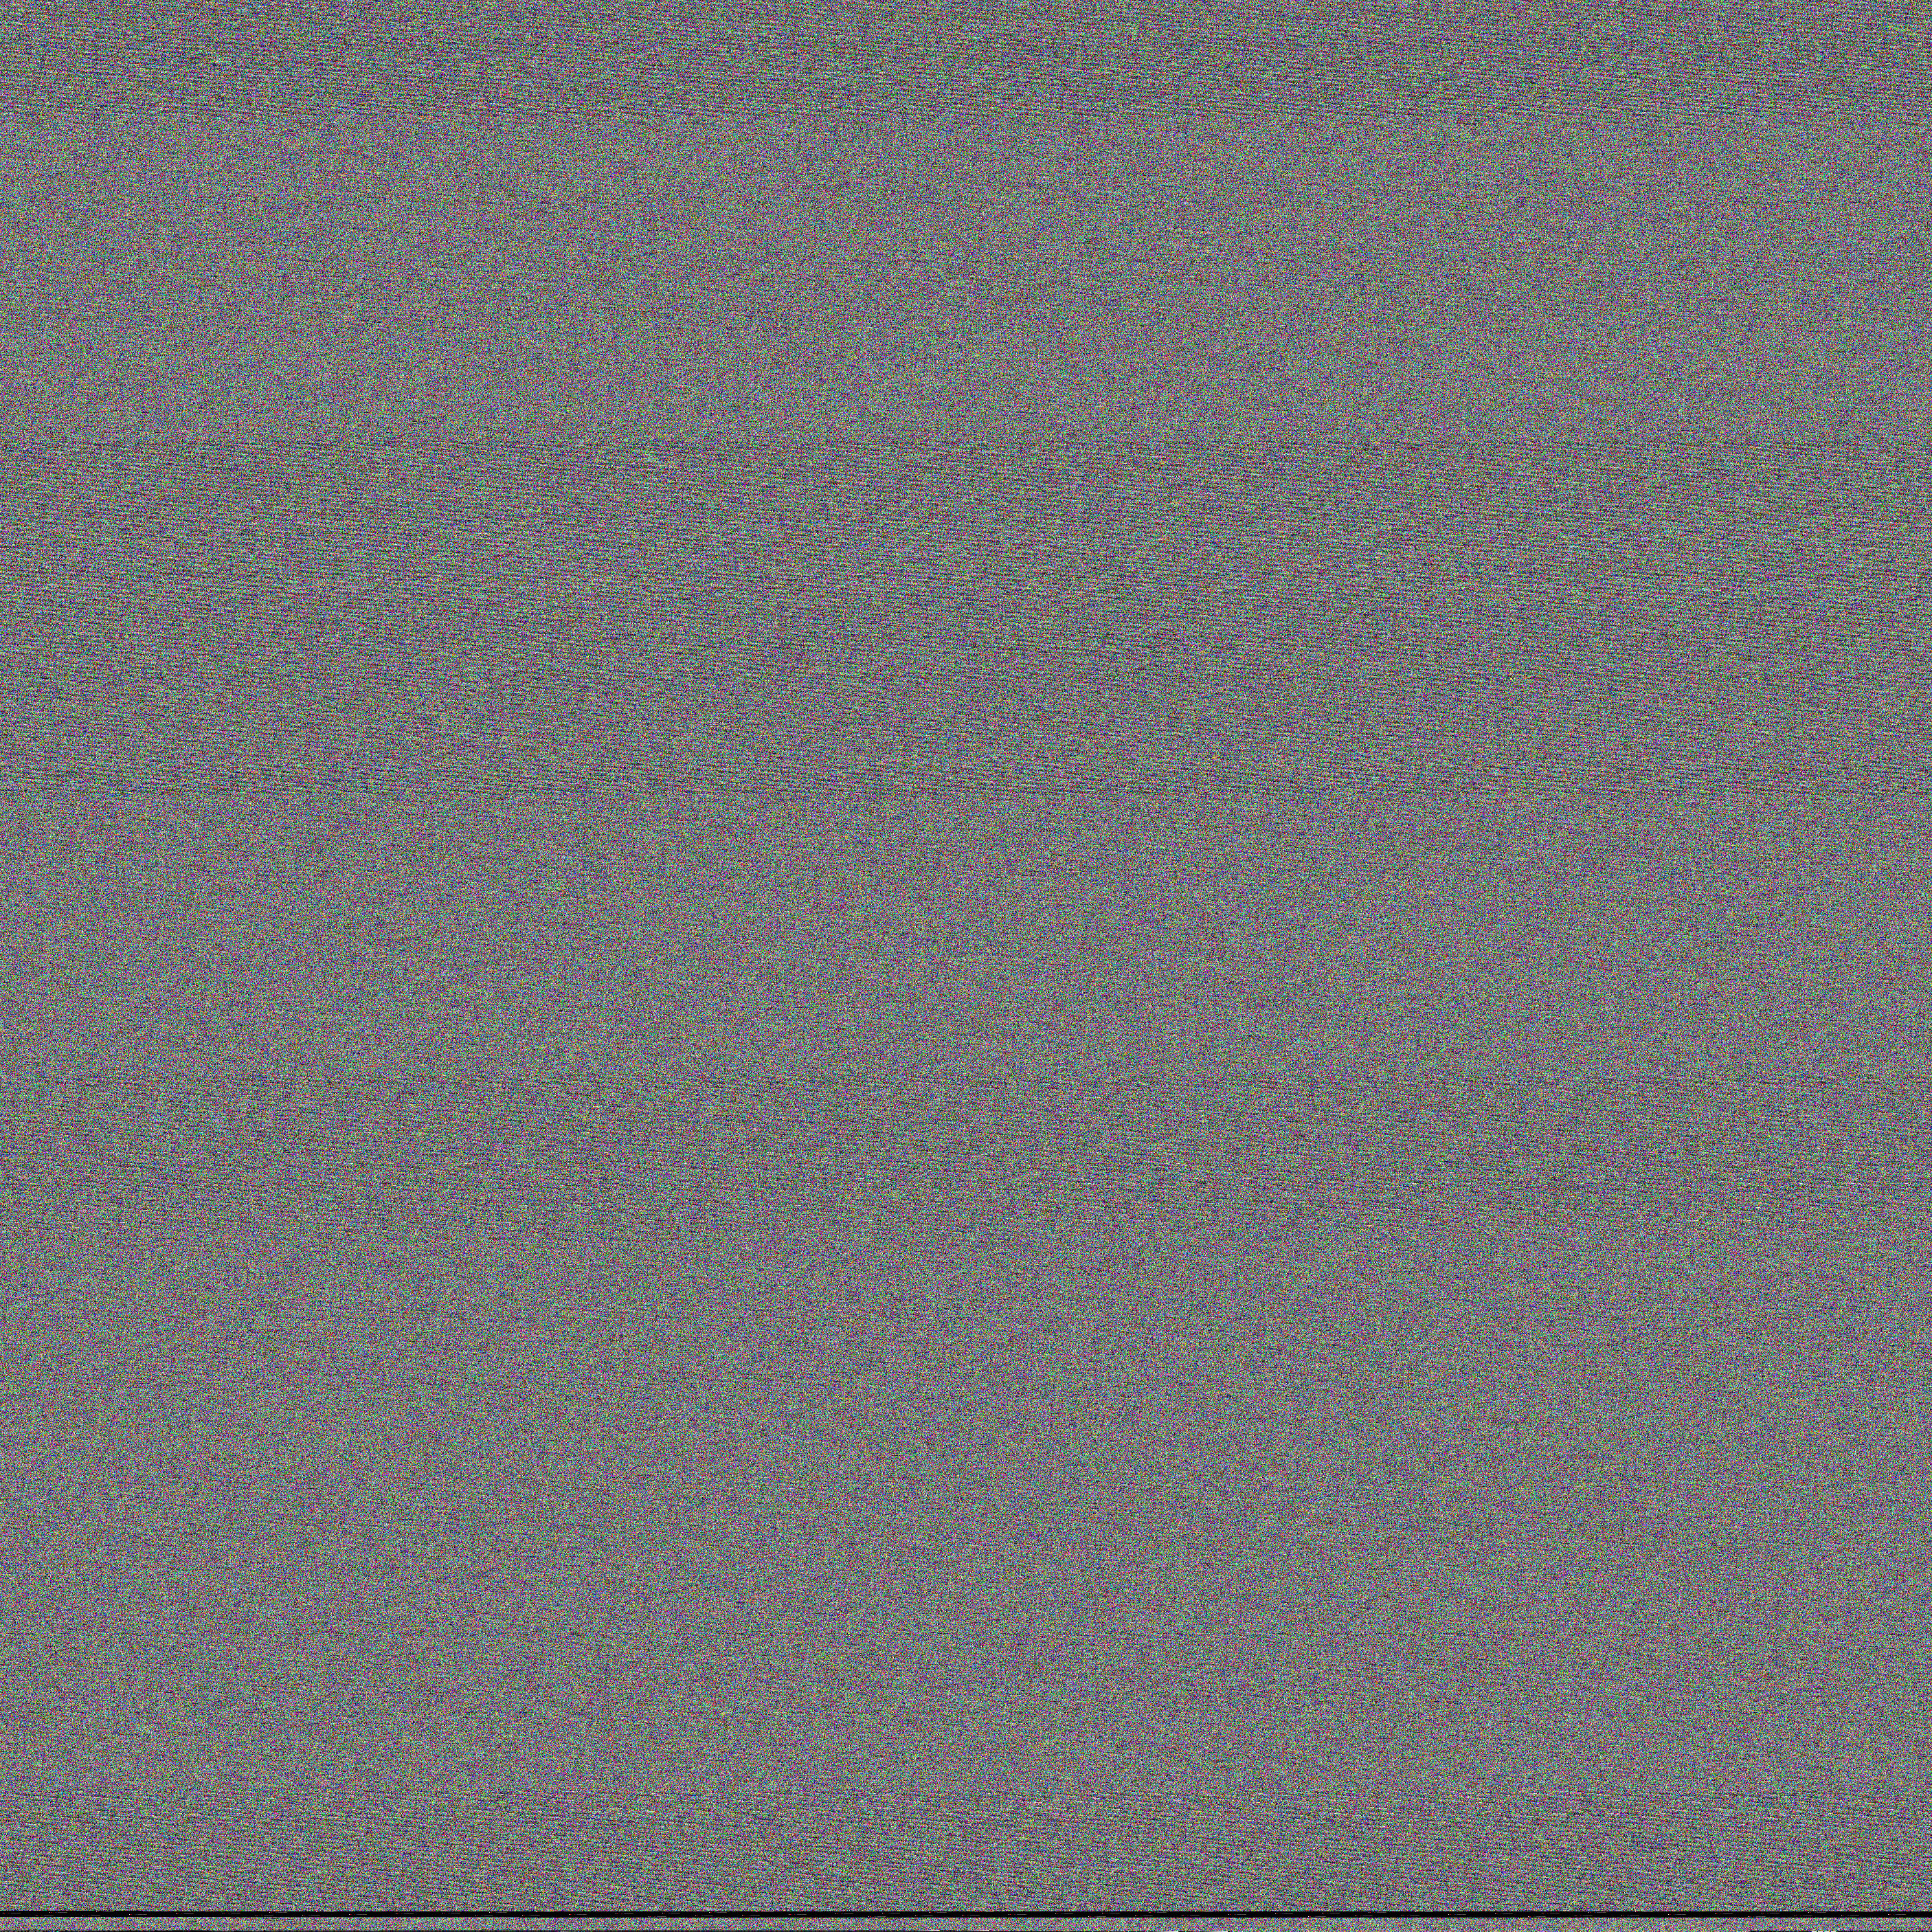
\includegraphics[width=0.3\textwidth]{imgs/proyecto0/outPNG-mp3}}
\\
\end{tabular}
\caption{Imágenes obtenidas de un binario .mp3}
\label{F:mp3}
\end{figure}

\begin{figure}[H]
\centering
\begin{tabular}{c c c}
\subfloat[Imagen en formato JPG]
{\includegraphics[width=0.3\textwidth]{imgs/proyecto0/outPNG-bmp}}
&
\subfloat[Imagen en formato PNG]
{\includegraphics[width=0.3\textwidth]{imgs/proyecto0/outJPG-bmp}}
&
\subfloat[Imagen en formato BMP]
{\includegraphics[width=0.3\textwidth]{imgs/proyecto0/outPNG-bmp}}
\\
\end{tabular}
\caption{Imágenes obtenidas de un binario .bmp}
\label{F:bmp}
\end{figure}

%%%%%%%%%%%%%%%%%%%%%%%%%%%%%%%%%%%%%%%%%%%%%%%%%%%%%%%%%%%%%%
% --> ANÁLISIS DE TIEMPOS DE EJECUCIÓN 
%%%%%%%%%%%%%%%%%%%%%%%%%%%%%%%%%%%%%%%%%%%%%%%%%%%%%%%%%%%%%%
\section{Análisis de tiempos de ejecución} 

Al ejecutar el código y crear las imágenes en los distintos formatos se calcula el tiempo de ejecución de cada algoritmo. Se realizaron diez mediciones, y de esta se sacó el promedio que tardó cada función. Se puede notar que la creación de las imágenes en formato BMP y JPEG tienen tiempos muy parecidos, alrededor de 4 segundos. Curiosamente, la creación de la imagen PNG tardó mucho más, un promedio de 21 segundos. La diferencia entre estos tiempos de ejecución está relacionada directamente con la compresión que utiliza cada formato; así como las funciones internas no estudiadas de cada biblioteca utilizada.

\begin{table}[H]
\begin{center}
    \begin{tabular}{ |>{\centering\arraybackslash}m{3cm}|>{\centering\arraybackslash}m{3cm}|>{\centering\arraybackslash}m{3cm}|>{\centering\arraybackslash}m{3cm}| }
    	\hline
    	\cellcolor{cl} \textbf{Tiempo} & \cellcolor{cl} \textbf{BMP} & \cellcolor{cl} \textbf{PNG}  & \cellcolor{cl} \textbf{JPG} \\ \hline \hline
        $T_1$ & 4,38060 & 20,21500 & 4,44193 \\ \hline
        $T_2$ & 4,67325 & 19,40460 & 5,91329 \\ \hline
        $T_3$ & 4,42406 & 24,98370 & 2,36694 \\ \hline
        $T_4$ & 4,34032 & 20,21500 & 2,48694 \\ \hline
        $T_5$ & 4,89789 & 27,75670 & 2,99915 \\ \hline
        $T_6$ & 4,31651 & 19,26920 & 8,54429 \\ \hline
        $T_7$ & 4,22170 & 19,00760 & 1,88674 \\ \hline
        $T_8$ & 4,57719 & 23,82840 & 2,23887 \\ \hline
        $T_9$ & 4,30820 & 21,26630 & 1,95731 \\ \hline
     $T_{10}$ & 4,28089 & 20,12690 & 5,81021 \\ \hline
        \textbf{Prom} & \textbf{4,94206} & \textbf{21,65671 } & \textbf{3,386453} \\ \hline
    \end{tabular}
\end{center}
\label{T:Time}
\caption{Resumen de características de los formatos de imágenes. \cite{R1}}
\end{table}




%%%%%%%%%%%%%%%%%%%%%%%%%%%%%%%%%%%%%%%%%%%%%%%%%%%%%%%%%%%%%%
% --> CONCLUSIONESS 
%%%%%%%%%%%%%%%%%%%%%%%%%%%%%%%%%%%%%%%%%%%%%%%%%%%%%%%%%%%%%%
\section{Conclusiones} 

Como conclusiones se tiene que:
\begin{itemize}
    \item Se logró entender la compresión y el formato de PNG, BMP, JPEG.
    \item Se comprende el modelo de color RGB.
    \item Se logra la lectura en binario permite obtener información en bits y darle cualquier formato para su uso.
     \item Utilización de  bibliotecas de terceros con buena documentación.
    \item Se comprendió cómo se enlazan bibliotecas estáticamente con la creación del programa
\end{itemize}

%%%%%%%%%%%%%%%%%%%%%%%%%%%%%%%%%%%%%%%%%%%%%%%%%%%%%%%%%%%%%%
% --> BIBLIOGRAFIA
%%%%%%%%%%%%%%%%%%%%%%%%%%%%%%%%%%%%%%%%%%%%%%%%%%%%%%%%%%%%%%
\begin{thebibliography}{IEEE}
\bibitem{R1} Luca, M. \textbf{\textit{A Basic Summary of Image Formats}}.  Visto el 5 de Mayo del 2018 en: \url{http://www.student.montefiore.ulg.ac.be/~merciadri/docs/papers/image-formats.pdf}.

\bibitem{R2} Autor Desconocido. \textbf{\textit{Digital images and image formats}}. Visto el 5 de Mayo del 2018 en: \url{http://www.uio.no/studier/emner/matnat/math/MAT-INF1100/h08/kompendiet/images.pdf}.

\bibitem{R3} Brown, A. \textbf{\textit{Graphics File Formats}}. 2008. THe National Archives. Visto el 5 de Mayo del 2018 en: \url{https://www.nationalarchives.gov.uk/documents/graphic-file-formats.pdf}.

\bibitem{R4} PNG. \textit{\textbf{Official documentation of libpng}}. Visto el 5 de Mayo del 2018 en: \url{http://www.libpng.org/pub/png/libpng.html}. 

\bibitem{R5} Kumar, T. Verma, K. \textbf{\textit{A Theory Based on Conversion of RGB image to Gray
image}}. 2010. International Journal of Computer Applications, Vol. 7. No. 2. Visto el 5 de Mayo del 2018 en: \url{https://www.researchgate.net/profile/Karun_Verma/publication/46286639_A_Theory_Based_on_Conversion_of_RGB_image_to_Gray_image/links/5704a3b008ae44d70ee0662c.pdf}.

\bibitem{R6} Greensted, A. \textbf{\textit{Creating PNGs with libpng}}. Visto el 5 de Mayo del 2018 en: \url{http://www.labbookpages.co.uk/software/imgProc/libPNG.html}.

\bibitem{R7} Autor Desconocido. \textbf{\textit{C++ Binary File I/O}}. Visto el 5 de Mayo del 2018 en: \url{http://courses.cs.vt.edu/~cs2604/fall00/binio.html}

\bibitem{R8} Raymon, E. \textbf{\textit{Introduction to GIFLIB}}. Visto el 5 de Mayo del 2018 en: \url{http://giflib.sourceforge.net/intro.html}

\bibitem{R9} Autor desconocido. \textbf{\textit{Magick::Image Class}}. Visto el 5 de Mayo del 2018 en: \url{https://www.imagemagick.org/api/Image++.php}

\end{thebibliography}
-
